\section{Информационно-логическая модель}\label{sec:infological-model}

\subsection{Информационные объекты}\label{subsec:information-objects}

Выделим следующие информационные объекты:
\begin{enumerate}
    \item \textbf{Тариф} \\
    Тариф -- это включаемые услуги и ставки оплаты за эти же услуги, предоставляемые компанией. Этот объект характеризуется следующими атрибутами:
    \begin{enumerate}
        \item Название:
        \begin{itemize}
            \item является уникальным идентификатором тарифа;
            \item разрабатывается менеджером (или группой менеджеров) компании сотового оператора;
            \item тип -- текстовый, максимальный размер -- 64 символа;
            \item используется как обозначение тарифа;
            \item администратор имеет доступ для чтения и записи, продавец-консультант и пользователь имеют только доступ для чтения.
        \end{itemize}

        \item Абонентская плата:
        \begin{itemize}
            \item является размером платы за тариф;
            \item разрабатывается менеджером (или группой менеджеров) компании сотового оператора;
            \item тип -- числовой, интервал возможных значений -- $[150; 5000]$;
            \item используется как описание размера платы за тариф;
            \item администратор имеет доступ для чтения и записи, продавец-консультант и пользователь имеют только доступ для чтения.
        \end{itemize}

        \item Интернет трафик:
        \begin{itemize}
            \item является размером предоставляемой компанией соответствующей услуги;
            \item разрабатывается менеджером (или группой менеджеров) компании сотового оператора;
            \item тип -- числовой, интервал возможных значений -- $[0; \infty]$; % или же обозначить бесконечность как -1
            \item используется как описание размер предоставляемой компанией соответствующей услуги;
            \item администратор имеет доступ для чтения и записи, продавец-консультант и пользователь имеют только доступ для чтения.
        \end{itemize}

        \item Количество минут:
        \begin{itemize}
            \item является размером предоставляемой компанией соответствующей услуги;
            \item разрабатывается менеджером (или группой менеджеров) компании сотового оператора;
            \item тип -- целочисленный, интервал возможных значений -- $[0; \infty]$; % или же обозначить бесконечность как -1
            \item используется как описание размер предоставляемой компанией соответствующей услуги;
            \item администратор имеет доступ для чтения и записи, продавец-консультант и пользователь имеют только доступ для чтения.
        \end{itemize}

        \item Количество SMS:
        \begin{itemize}
            \item является размером предоставляемой компанией соответствующей услуги;
            \item разрабатывается менеджером (или группой менеджеров) компании сотового оператора;
            \item тип -- целочисленный, интервал возможных значений -- $[0; \infty]$; % или же обозначить бесконечность как -1
            \item используется как описание размер предоставляемой компанией соответствующей услуги;
            \item администратор имеет доступ для чтения и записи, продавец-консультант и пользователь имеют только доступ для чтения.
        \end{itemize}
    \end{enumerate}

    \begin{figure}[H]
        \label{fig:tariff-objects}
        \caption{Взаимосвязи атрибутов объекта <<Тариф>>}
        \center{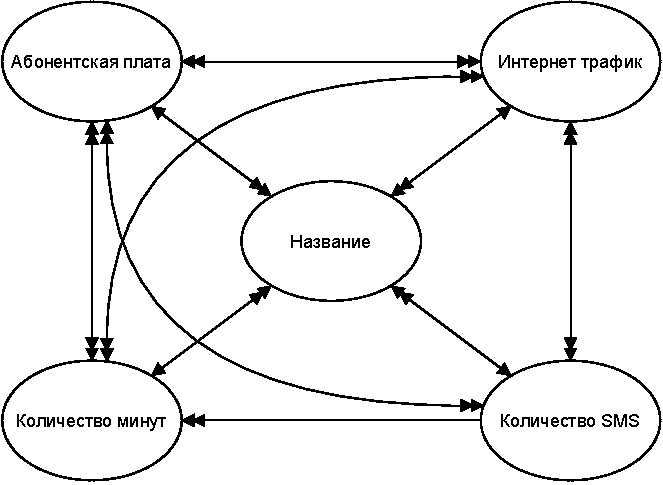
\includegraphics{graphics/tariff-objects}}
    \end{figure}

    \item \textbf{SIM-карта} \\
    SIM-карта -- это идентификационный электронный модуль мобильной связи сотового оператора. Этот объект характеризуется следующими атрибутами:
    \begin{enumerate}
        \item Расчётный счёт:
        \begin{itemize}
            \item является номером банковского счёта;
            \item выдаётся банком, с которым сотовый оператор состоит в партнёрских отношениях;
            \item тип -- целочисленный, интервал возможных значений -- $[10000000000000000000; 99999999999999999999]$;
            \item используется как номер банковского счёта для оплаты за услуги;
            \item администратор, продавец-консультант и пользователь имеют только доступ для чтения.
        \end{itemize}

        \item Телефонный номер:
        \begin{itemize}
            \item является идентификационным номером в телекоммуникационной системе связи;
            \item получает компания сотового оператора;
            \item тип -- целочисленный, интервал возможных значений -- $[70000000000; 79999999999]$;
            \item используется как номер идентификационный номер в телекоммуникационной системе связи;
            \item администратор, продавец-консультант и пользователь имеют только доступ для чтения.
        \end{itemize}

        \item Зарегистрированный тариф:
        \begin{itemize}
            \item ...
        \end{itemize}
    \end{enumerate}

    \item \textbf{Абонент} \\
    Абонент -- это пользователь услугами сотового оператора. Этот объект является наиболее важным пользователем в системе. Абонент характеризуется следующими аттрибутами:
    \begin{enumerate}
        \item фамилия абонента;
        \item имя абонента;
        \item отчество абонента;
        \item номер паспорта
    \end{enumerate}
\end{enumerate}